\section{Seguimiento}

El seguimiento de trayectoria se realiza sobre una ventana deslizante de tres a cuatro cuadros donde se enlazan los puntos reconstruidos de manera de mantener un movimiento lo mas suave posible debido a la hipótesis que el muestreo permite observar una evolución lenta con desplazamiento mínimo entre cuadros.

Esta metodología fue la utilizada por Herda \cite{herda} en su trabajo basándose en los estudios de Malik, Drako, Papantoniou \cite{griegos} .

\subsection{Algoritmo}

Sea una trayectoria de un marcador enlazada hasta el instante [f] la cual desea buscarse su próximo punto en [f+1], el movimiento entre [f-1] y [f] es prolongado en dirección y modulo para establecer un centro de búsqueda para encontrar el punto reconstruido que mejor continúa la trayectoria en un proceso mostrado en la Figura \ref{herda_00} .

\begin{figure}[ht!]
\begin{center}
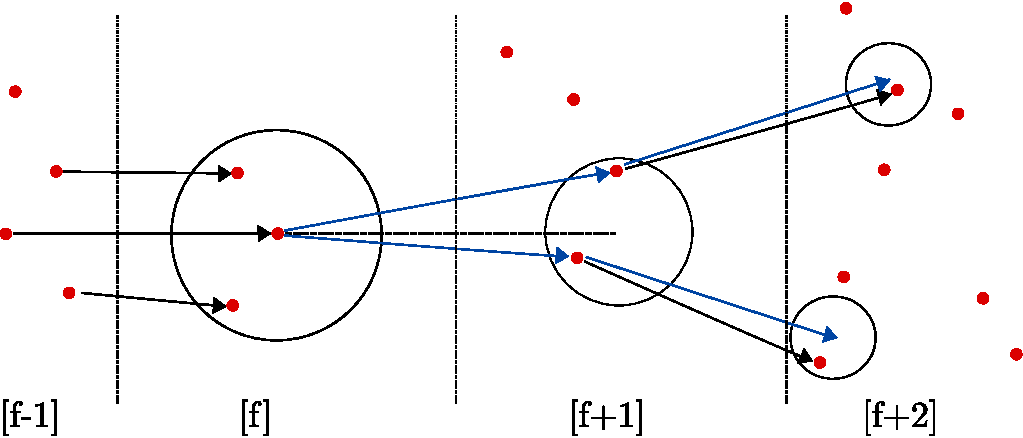
\includegraphics[scale=0.6]{imagenes/Seguimiento/tracking-eps-converted-to.pdf}
\end{center}
\caption{Seguimiento en cuatro cuadros, siendo [f] el cuadro actual que queremos seguir en [f+1]. ( Fuente  Human movement
science 20(3), 313–341 \cite{herda} ) .}
\label{herda_00}
\end{figure}

Se presentan tres posibles casos al buscar puntos reconstruidos:

\begin{itemize}

\item Si solo se encuentra un punto reconstruido dentro de la búsqueda se agrega a la trayectoria para el cuadro [f+1], mientras mas cercano se encuentre a la estimación calculada como aquella que mejor se aproxima a una trayectoria de tres puntos con aceleración mínima

\item En el caso de encontrar mas de un punto dentro del radio de búsqueda cada posible candidato es utilizado para realizar una segunda estimación hacia [f+2] de forma que la aceleración entre [f-1], [f] y el candidato en [f+1] sea la misma que entre [f], el candidato en [f+1] y la estimación en [f+2] (el radio de búsqueda en [f+2] corresponde a la distancia entre el candidato en [f+1] y la estimación en [f+2]). Luego de todos los posible caminos en cuatro cuadros, se elige el de menor variación de aceleración.

\item Si no se encuentra ningún punto, se procede a aumentar acotadamente el radio de búsqueda en [f+1] de forma excepcional. Esto se hace para continuar trayectorias que entran en estado de reposo y el ultimo movimiento conocido es nulo o muy pequeño.

\end{itemize}

Si una trayectoria queda trunca durante el enlazado, se intenta recuperar prolongando el movimiento en próximas cuadros para encontrar puntos reconstruidos cercanos a las estimaciones y extrapolar los puntos intermedios. Por otro lado, se implementan umbrales para definir limites sobre la aceleración de los enlaces obtenidos y detectar discontinuidades durante el seguimiento.

Con estas medidas implementadas es posible detectar las trayectorias individuales sobre los puntos reconstruidos, detectar de forma simple posibles discontinuidades, y estimar reemplazos en casos de perdidas. La captura mostrada en la Figura \ref{restricciones_tracking} corresponde a la marcha y se resalta las trayectorias individuales de puntos de la pierna así como un esqueleto simple generado simplemente para visualizar la evolución entre marcadores

\begin{figure}[ht!]
 \hspace{-1.3cm}
  \subfloat[Trayectorias de marcadores de pierna.]{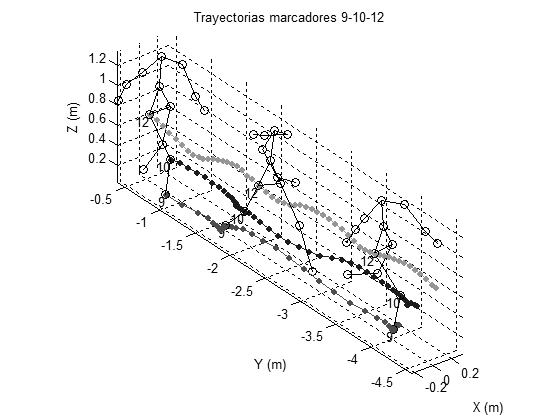
\includegraphics[scale=0.4]{imagenes/Seguimiento/050_Salida_Tracking_13_14_10.png} %\label{trayectorias_marcadores_piernas}
   }	
  \subfloat[Distancia y Angulo entre marcadores de la pierna.]{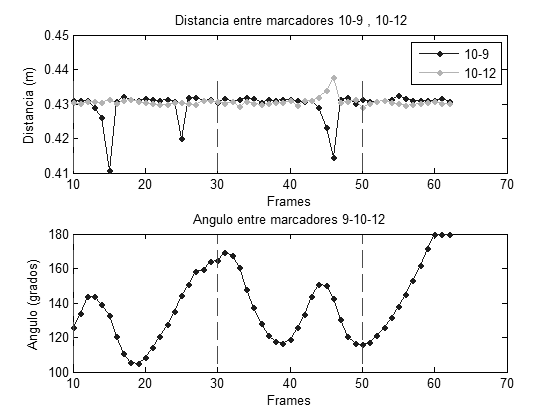
\includegraphics[scale=0.4]{imagenes/Seguimiento/051_Salida_Angulo_Distancia_13_14_10.png}\label{distancia_angulo_marcadores_piernas}}
\caption{Posibles restricciones en ángulo y distancia, para el caso de la pierna en marcha.}
\label{restricciones_tracking}
\end{figure}

El conjunto de puntos reconstruidos puede ser sometido a otros algoritmos de seguimiento como por Kalman \cite{kalman} requiriendo la inicialización de modelos, o algoritmos basados en restricciones mas fuertes a las presentadas en este trabajo como podrían ser las distancias relativamente constantes entre marcadores de los miembros y ángulos continuos entre articulaciones pero requieren un estudio considerable de las características de cada sujeto y movimiento a capturar. La Figura \ref{restricciones_tracking} muestra algunas posibles restricciones en la marcha sobre los huesos de la pierna.

